\documentclass[landscape]{article}
\usepackage[a4paper,landscape,margin=1.5cm]{geometry}
\usepackage{graphicx}
\usepackage{array}
\usepackage{tabularx}
\usepackage{colortbl}
\usepackage{xcolor}
\usepackage{fancyhdr}
\usepackage{tikz}
\usepackage{booktabs}
\usepackage{subcaption}
\usepackage{pagecolor}

\graphicspath{{illustration/}{reference/}}  % DO NOT CHANGE THIS LINE

% Define custom colors
\definecolor{headerblue}{RGB}{0,0,0}
\definecolor{lightgray}{RGB}{240,240,240}
\definecolor{lightbeige}{RGB}{252,250,245} % Light beige color
\pagecolor{lightbeige} % Set background color

% Custom page style
\pagestyle{fancy}
\fancyhf{}
\renewcommand{\headrulewidth}{0pt}
\cfoot{\textcolor{headerblue}{\thepage}} % Added page number in footer center

\begin{document}
% Header Section
\begin{center}
\Huge\bfseries\sffamily\textcolor{headerblue}{TECHNICAL SPECIFICATION SHEET}
\end{center}

\vspace{0.5cm}

% PRODUCT DETAILS
\noindent\begin{tabularx}{\textwidth}{|X|X|X|X|}
\hline
\rowcolor{headerblue}\multicolumn{4}{|c|}{\textcolor{white}{\textbf{PRODUCT DETAILS}}} \\
\hline
Brand Name: E & Designer: W & Season: Autumn/Winter & Category: Outerwear \\
\hline
Date: March 2025 & Style Name: Elegant Black Coat & Style Number: 001 & Main Fabric: Wool \\
\hline
\end{tabularx}

\vspace{0.5cm}

% STYLE DESCRIPTION
\noindent\begin{tabularx}{\textwidth}{|X|}
\hline
\rowcolor{headerblue}\multicolumn{1}{|c|}{\textcolor{white}{\textbf{STYLE DESCRIPTION}}} \\
\hline
An elegant black coat featuring a tailored fit with clean lines, designed for a sophisticated look. The coat is crafted from high-quality wool, offering warmth and comfort, perfect for the cooler months.
\end{tabularx}
\hline

\vspace{0.5cm}

% TECHNICAL DRAWINGS
\noindent\begin{tabularx}{\textwidth}{|X|}
\hline
\rowcolor{headerblue}\multicolumn{1}{|c|}{\textcolor{white}{\textbf{TECHNICAL DRAWINGS}}} \\
\hline
\begin{center}
% First row of drawings
\begin{tabular}{c}
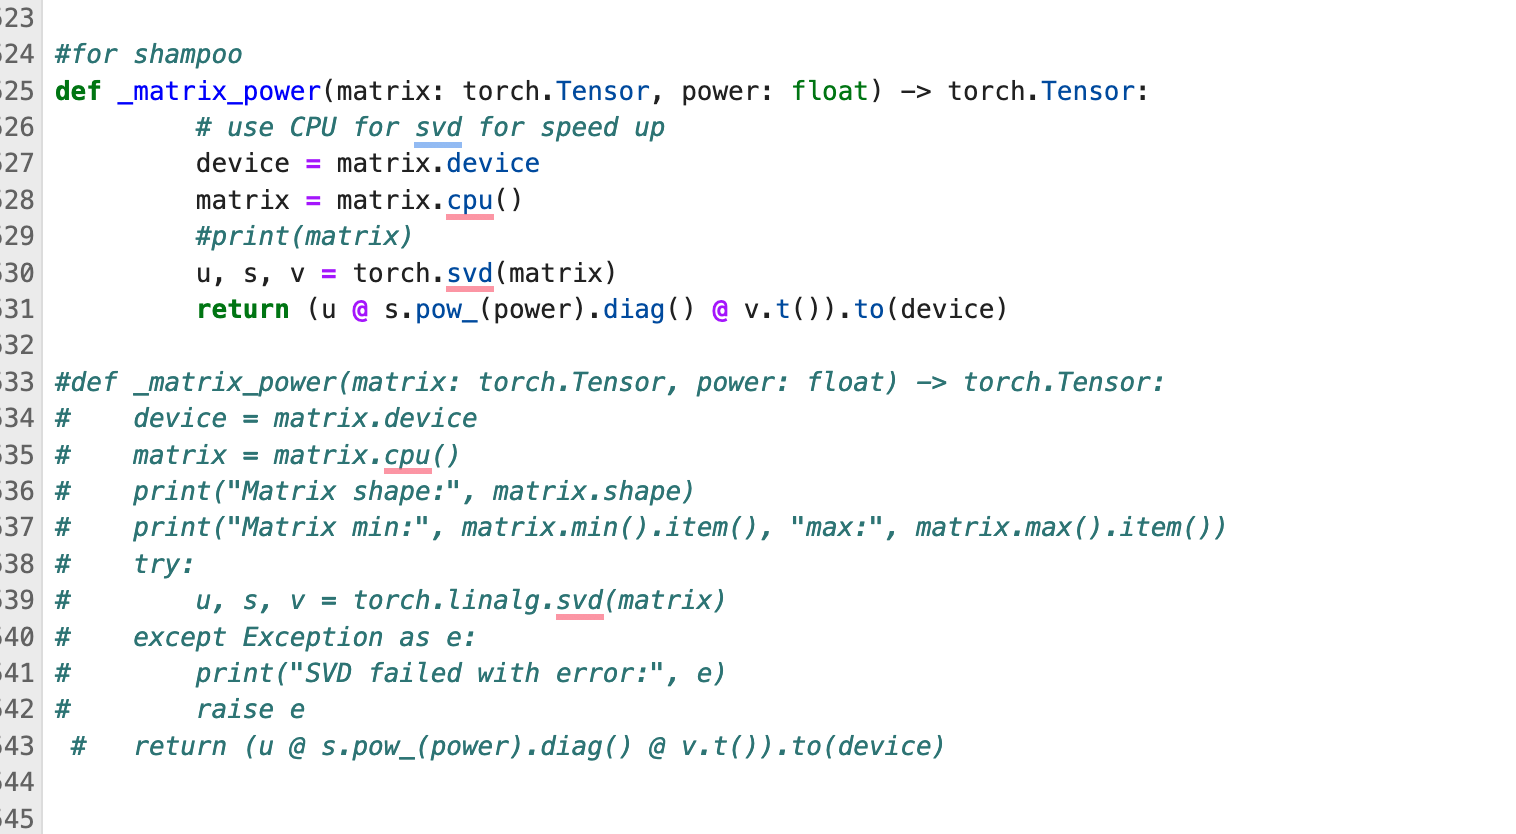
\includegraphics[width=0.4\textwidth,height=8cm,keepaspectratio]{Screenshot_2025-03-09_at_15.26.02.png} \\
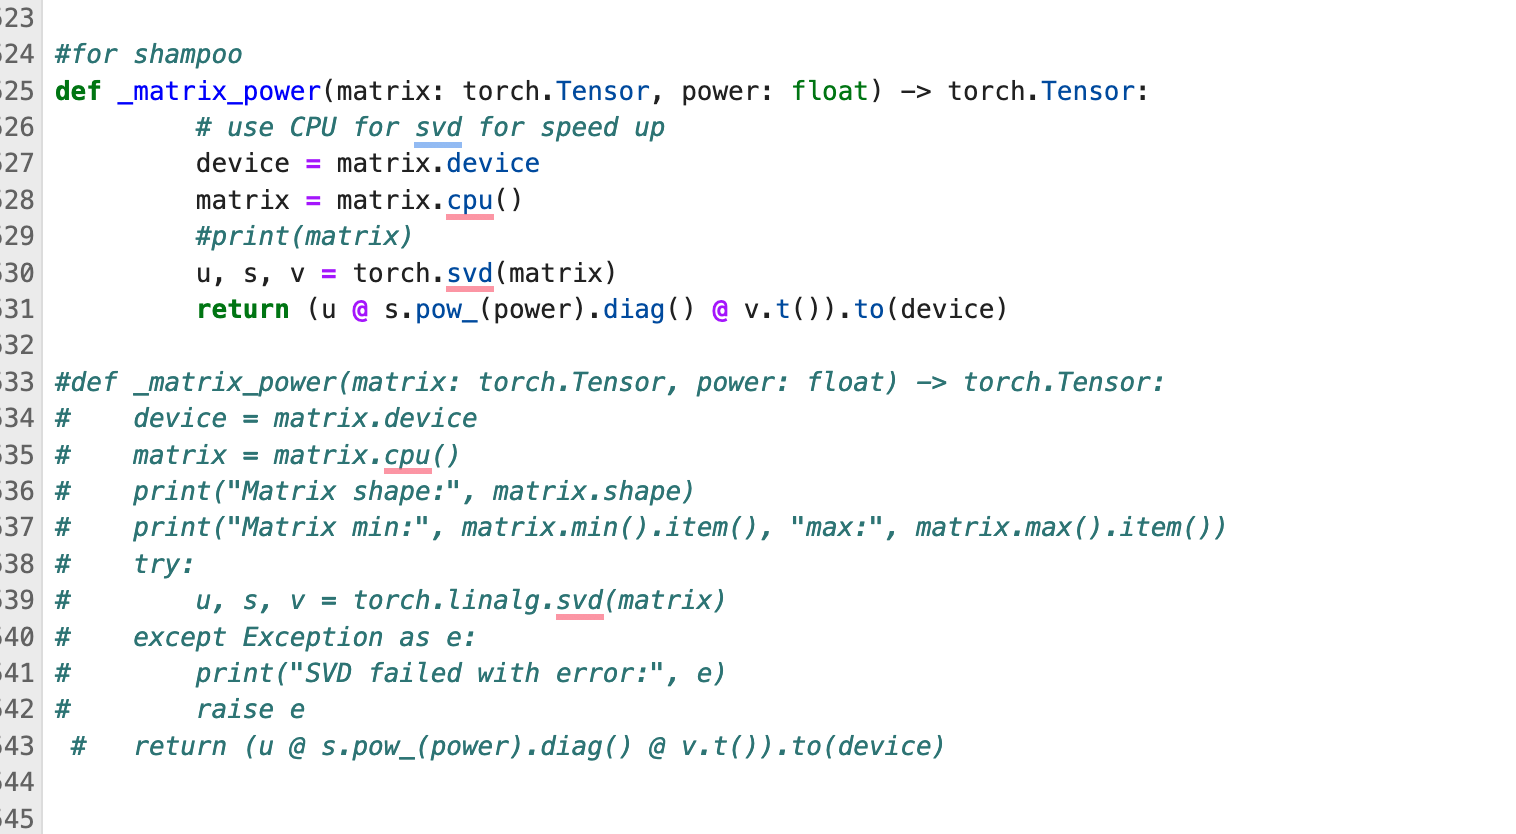
\includegraphics[width=0.4\textwidth,height=8cm,keepaspectratio]{Screenshot_2025-03-09_at_15.26.02.png} \\
\end{tabular}
\end{center}
\end{tabularx}
\hline

\vspace{0.5cm}

\newpage
% MEASUREMENTS
\noindent\begin{tabularx}{\textwidth}{|X|X|X|X|X|X|X|}
\hline
\rowcolor{headerblue}\multicolumn{7}{|c|}{\textcolor{white}{\textbf{MEASUREMENTS}}} \\
\hline
\textbf{Item} & \textbf{Description} & \textbf{XS} & \textbf{S} & \textbf{M} & \textbf{L} & \textbf{XL}\\
\hline
Shoulder Width & Distance between shoulder seams, wool & 40 cm & 42 cm & 44 cm & 46 cm & 48 cm \\
\hline
Chest Width & Across the chest, wool & 92 cm & 96 cm & 100 cm & 104 cm & 108 cm \\
\hline
Sleeve Length & From shoulder to cuff, wool & 60 cm & 61 cm & 62 cm & 63 cm & 64 cm \\
\hline
Total Length & From top of shoulder to hem, wool & 100 cm & 102 cm & 104 cm & 106 cm & 108 cm \\
\hline
\end{tabularx}

\vspace{0.5cm}

% CARE INSTRUCTIONS
\noindent\begin{tabularx}{\textwidth}{|X|}
\hline
\rowcolor{headerblue}\multicolumn{1}{|c|}{\textcolor{white}{\textbf{CARE INSTRUCTIONS}}} \\
\hline
\begin{itemize}
    \item Dry clean only.
    \item Do not bleach.
    \item Iron at low temperature if needed, using a protective cloth.
    \item Store in a cool, dry place away from direct sunlight.
    \item Avoid contact with rough surfaces to prevent snagging.
\end{itemize}
\end{tabularx}
\hline

\vspace{0.5cm}

% ADDITIONAL COMMENTS
\noindent\begin{tabularx}{\textwidth}{|X|}
\hline
\rowcolor{headerblue}\multicolumn{1}{|c|}{\textcolor{white}{\textbf{ADDITIONAL COMMENTS}}} \\
\hline
this is super good.
\end{tabularx}
\hline

\newpage
% ABOUT TECH PACKS
\noindent\begin{tabularx}{\textwidth}{|X|}
\hline
\rowcolor{headerblue}\multicolumn{1}{|c|}{\textcolor{white}{\textbf{ABOUT TECH PACKS}}} \\
\hline
Tech packs are indispensable tools in the fashion industry, providing a comprehensive blueprint for garment production. They contain all necessary details such as technical specifications, measurements, materials, colors, and construction methods, ensuring that the designer's vision is accurately translated into the final product. By serving as a communication bridge between designers and manufacturers, tech packs help streamline the production process, minimize errors, and reduce costs. They also facilitate quality control and consistency across production runs by offering clear guidelines and standards. As living documents, tech packs are updated with design changes, making them crucial for adapting to new trends and requirements. In the context of new jacket designs, tech packs play a vital role in innovating and maintaining the garment's functionality, style, and comfort. The process of creating a tech pack starts with initial sketches and evolves through detailed illustrations, fabric selections, and precise measurements. A well-crafted tech pack can significantly impact the speed and efficiency of bringing a new jacket design to market while maintaining high standards of quality. This is particularly important in the competitive fashion industry, where time-to-market and adherence to design specifications are critical for success. Tech packs are not only about ensuring that the final product aligns with the designer's expectations but also about enhancing communication and collaboration across different teams involved in the production process. As the fashion industry continues to evolve with new technologies and sustainable practices, the role of tech packs will likely expand, incorporating digital tools and environmentally friendly materials. In summary, tech packs are essential for executing new jacket designs that meet consumer demands and align with the latest fashion trends. They provide a structured approach to garment production, ensuring that every aspect of the design is meticulously planned and executed. This comprehensive approach helps designers and manufacturers create innovative, high-quality jackets that stand out in the marketplace, ultimately contributing to the brand's reputation and success.
\end{tabularx}
\hline

\end{document}